\documentclass[conference]{IEEEtran}
%\documentclass{article}
\usepackage{footnote}
\usepackage[font={small}]{caption}
%\usepackage{sidecap}
\usepackage{graphicx}
\usepackage{cite}
\usepackage{hyperref}
%\usepackage[stable]{footmisc}
%\usepackage{caption}
%\usepackage{adjustbox}
\usepackage{subcaption}
\usepackage{algpseudocode}
\usepackage{algorithm}
\usepackage{amsmath}
\usepackage{amssymb}
\usepackage[T1]{fontenc}
\usepackage[utf8]{inputenc}
\usepackage{authblk}
\pdfminorversion=4

\title{Mirror Match: Reliable Feature Point Matching Without Geometric 
Constraints}

\author[1,2]{Jonas Toft Arnfred\thanks{j.arnfred@adsc.sg.com}}
\author[1]{Dr. Stefan Winkler\thanks{Stefan.Winkler@adsc.com.sg}}
\author[2]{Prof. Sabine S\"usstrunk\thanks{sabine.susstrunk@epfl.ch}}
\affil[1]{Advanced Digital Science Center, Singapore}
\affil[2]{\'Ecole Polytechnique F\'ed\'erale de Lausanne}

\begin{document}
\maketitle
%
\begin{abstract}
Many algorithms have been proposed to solve the problem of matching 
feature points in two or more images using geometric assumptions to 
increase the robustness of the matching. However, very little work 
addresses the case where these assumptions might not hold. In particular 
few methods address the problem of reliable matching in cases where it 
is unknown whether two images have any corresponding areas or objects in 
the first place. 

We propose two algorithms for matching feature points without the use of 
geometric constraints. The first relies on the fact that any match 
between two images should be better than all possible matches within a 
single image. The second algorithm extends this idea by using community 
structure in the similarity graph of feature points to find reliable 
correspondences. To evaluate the algorithms experimentally, we introduce 
a simple method to generate a large amount of test cases based on a set 
of image pairs with viewpoint changes. Our results show that the 
proposed algorithm is generally superior to traditional approaches in 
finding correct correspondences.
\end{abstract}
%
\section{Introduction}
%
When finding correspondence pairs between two or more images we are 
often faced with the problem that feature points in one image cannot be 
uniquely matched with feature points in another image. This is partly 
due to the fact that the discriminatory powers of modern feature 
descriptors such as \emph{SIFT} \cite{lowe2004sift} and \emph{SURF} 
\cite{bay2006surf} is reduced to approximate invariance to light and 
perspective changes.  Additionally corners detected by feature detectors 
such as \emph{SIFT} and \emph{Harris} \cite{harris1988combined} are only 
approximations of the ideal unique feature point in an image which is 
uniquely identifiable.  Both deficiencies often lead to a sub optimal 
matching when we match feature points by finding the nearest neighbors 
in terms of descriptor similarity. For this reason Lowe introduced a 
matching method tailored to find unique matches when he introduced the 
\emph{SIFT} feature point \cite{lowe2004sift}. The uniqueness of a given 
match is assessed by looking at the two nearest neighbors of each 
feature point and calculating the matching score as the ratio of 
similarities. The method, \emph{NN-Ratio} then matches feature points by 
matching each feature point with its nearest neighbor and only returning 
the matches which a ratio better than a given threshold. Compared to a 
nearest neighbor approach using the similarity of the descriptors as 
threshold, Lowe's \emph{NN-Ratio} performs better as shown by 
Mikolajczyk \cite{mikolajczyk2005performance}.

More recent methods for matching feature points consider the geometric 
configuration of feature points and match them based on assumptions 
about the geometric relationship between images.  These assumptions are 
then used to select a subset of matches according to different 
constraints e.g.\ angular constraints \cite{kim2008efficient}, epipolar 
constraints \cite{torr2000mlesac,chum2005matching}, or pairwise 
constraints \cite{choi2009robust,leordeanu2005spectral}.

Alternatively we can pick out different regions in each image and pair 
regions according to how many correspondences there are between them.  
This allows for the filtering of all correspondences that do not match 
points within paired regions.  Examples include \cite{das2008event} and 
\cite{wu2011robust}, the first (later referred to as \emph{Isodata}) 
uses clustering to find regions while the latter uses maximally stable 
extremal regions (MSER) to designate areas.

Solutions that make use of geometric assumptions about the images fall 
short in many practical applications. For example images with partial or 
no overlap often leads to feature points that match to arbitrary points 
in the other image leading to noise that makes it hard to pick the right 
subset of correct matches. Similarly adjacent objects in one image that 
are separated in another will void any global geometric assumptions of 
the geometric relationship between two images.  Furthermore, methods 
using geometric constraints all require an initial set of 
correspondences. If this set of correspondences can be narrowed down to 
the most probable correct matches, the geometric matching algorithm will 
benefit in terms of speed and accuracy in cases where geometric 
assumptions indeed hold true. For these reasons many applications call 
for reliable non geometric matching methods.

The two methods we propose in this paper are designed to be free of 
assumptions about the image geometry. They improve on Lowe's 
\emph{NN-Ratio} by attempting at matching only feature points that have 
a unique correspondence. The first algorithm, \emph{Mirror Match (MM)} 
is inspired by a simple but novel idea.  If a given feature point in one 
image is better matched with other feature points from the \emph{same} 
image than points in the other image, then any matches from this feature 
point to points in the other image are considered unreliable and should 
be discarded.  This approach carries no implicit assumptions about the 
geometric consistency of matches and as such can easily be extended with 
other geometric solutions when appropriate or necessary. \emph{Mirror 
Match with Clustering (MMC)} builds upon this idea by trying to group 
similar feature points and match them separately from the feature points 
that have unique correspondences. The experimental results show that 
both approaches generally outperform existing correspondence matching 
methods when tested on partially overlapping images.

The paper is organized as follows.  Section~\ref{S:MatchingMethods} 
describes the proposed \emph{Mirror Match (MM)} and \emph{Mirror Match 
with Clustering (MMC)} algorithms.  Section~\ref{S:Experiments} presents 
the dataset used for evaluation and the experimental setup.  
Section~\ref{S:Results} discusses the benchmarking results obtained.  
Section~\ref{S:Summary} concludes the paper.  

\section{Matching Methods}
\label{S:MatchingMethods}
%
\subsection{Mirror Match (\emph{MM})}
%
\begin{figure}
	\centering%
        \begin{subfigure}[t]{\columnwidth}
			\centering
			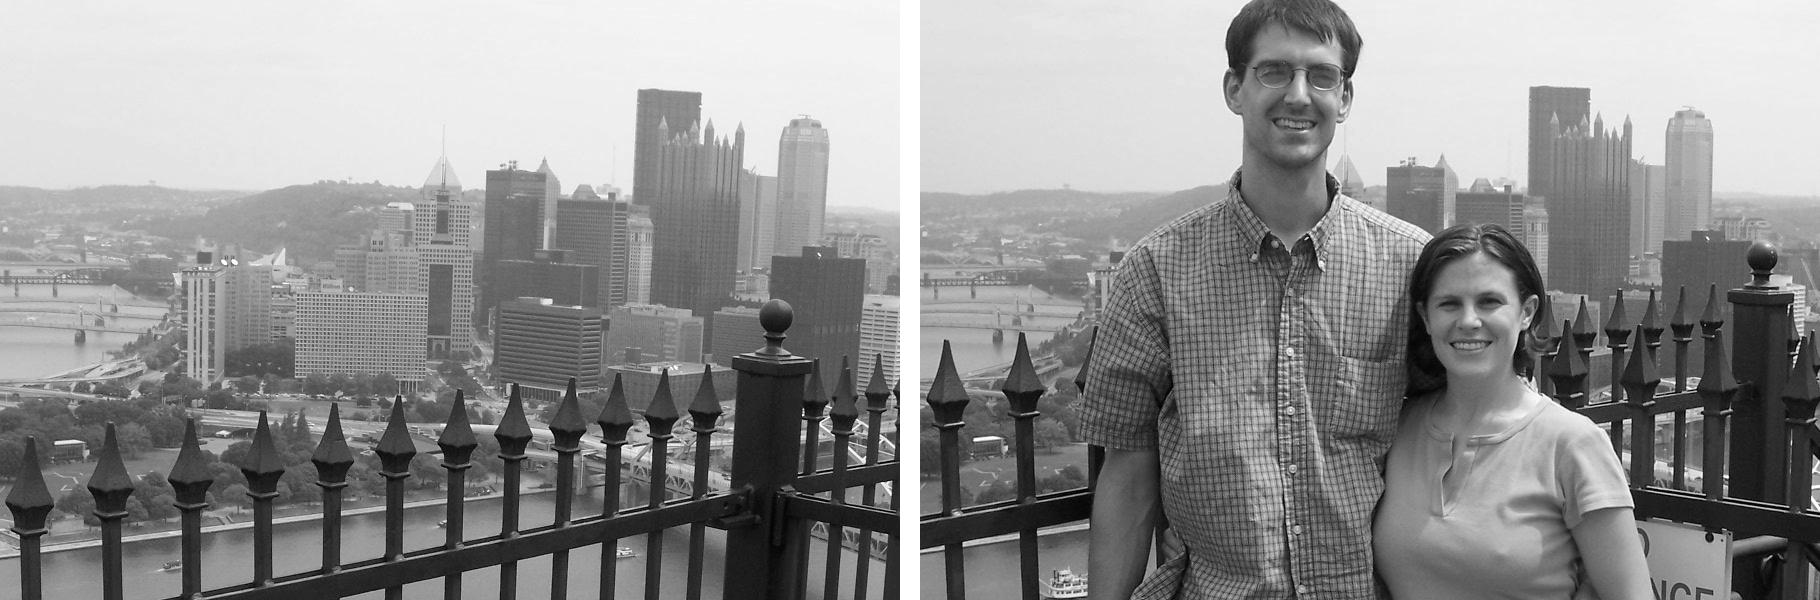
\includegraphics[width=0.85\columnwidth]{images/MMC_pitts_source}
			\caption{Source image pair}
			\label{fig:pitts_source}
		\end{subfigure}%
		\\ %
        \begin{subfigure}[t]{\columnwidth}
			\centering
			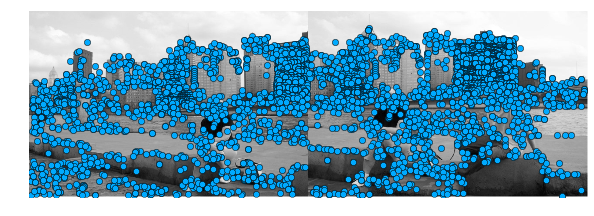
\includegraphics[width=0.85\columnwidth]{images/MMC_pitts_keypoints}
			\caption{Feature points}
			\label{fig:pitts_keypoints}
		\end{subfigure}%
		\\ %add desired spacing between images, e. g. ~, \quad, 
		%\qquad (or a blank line to force the subfigure onto a new line)
        \begin{subfigure}[t]{\columnwidth}
			\centering
			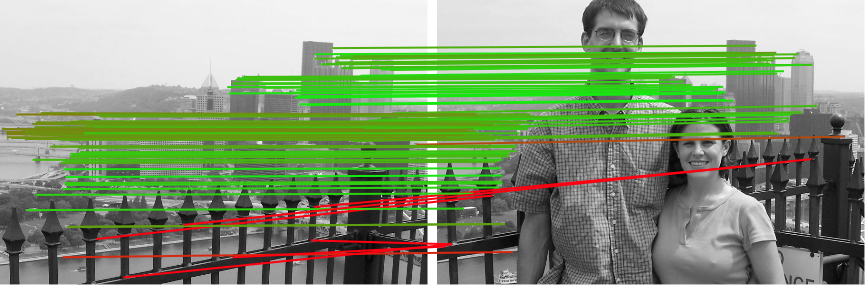
\includegraphics[width=0.85\columnwidth]{images/mirror_match_off}
            \caption{\emph{NN-Ratio}}
			\label{fig:unique}
		\end{subfigure}%
        \\ %add desired spacing between images, e. g. ~, \quad, 
        \begin{subfigure}[t]{\columnwidth}
			\centering
			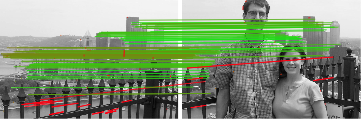
\includegraphics[width=0.85\columnwidth]{images/mirror_match_with_pruned}
			\caption{\emph{MM} intermediate result}
			\label{fig:within}
		\end{subfigure}%
		\\ %add desired spacing between images, e. g. ~, \quad, 
		%\qquad (or a blank line to force the subfigure onto a new line)
        \begin{subfigure}[t]{\columnwidth}
			\centering
			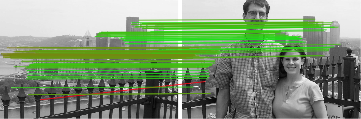
\includegraphics[width=0.85\columnwidth]{images/mirror_match}
			\caption{\emph{MM} final result}
			\label{fig:without}
		\end{subfigure}%
		\\ %add desired spacing between images, e. g. ~, \quad, 
		\begin{subfigure}[t]{\columnwidth}
			\centering
			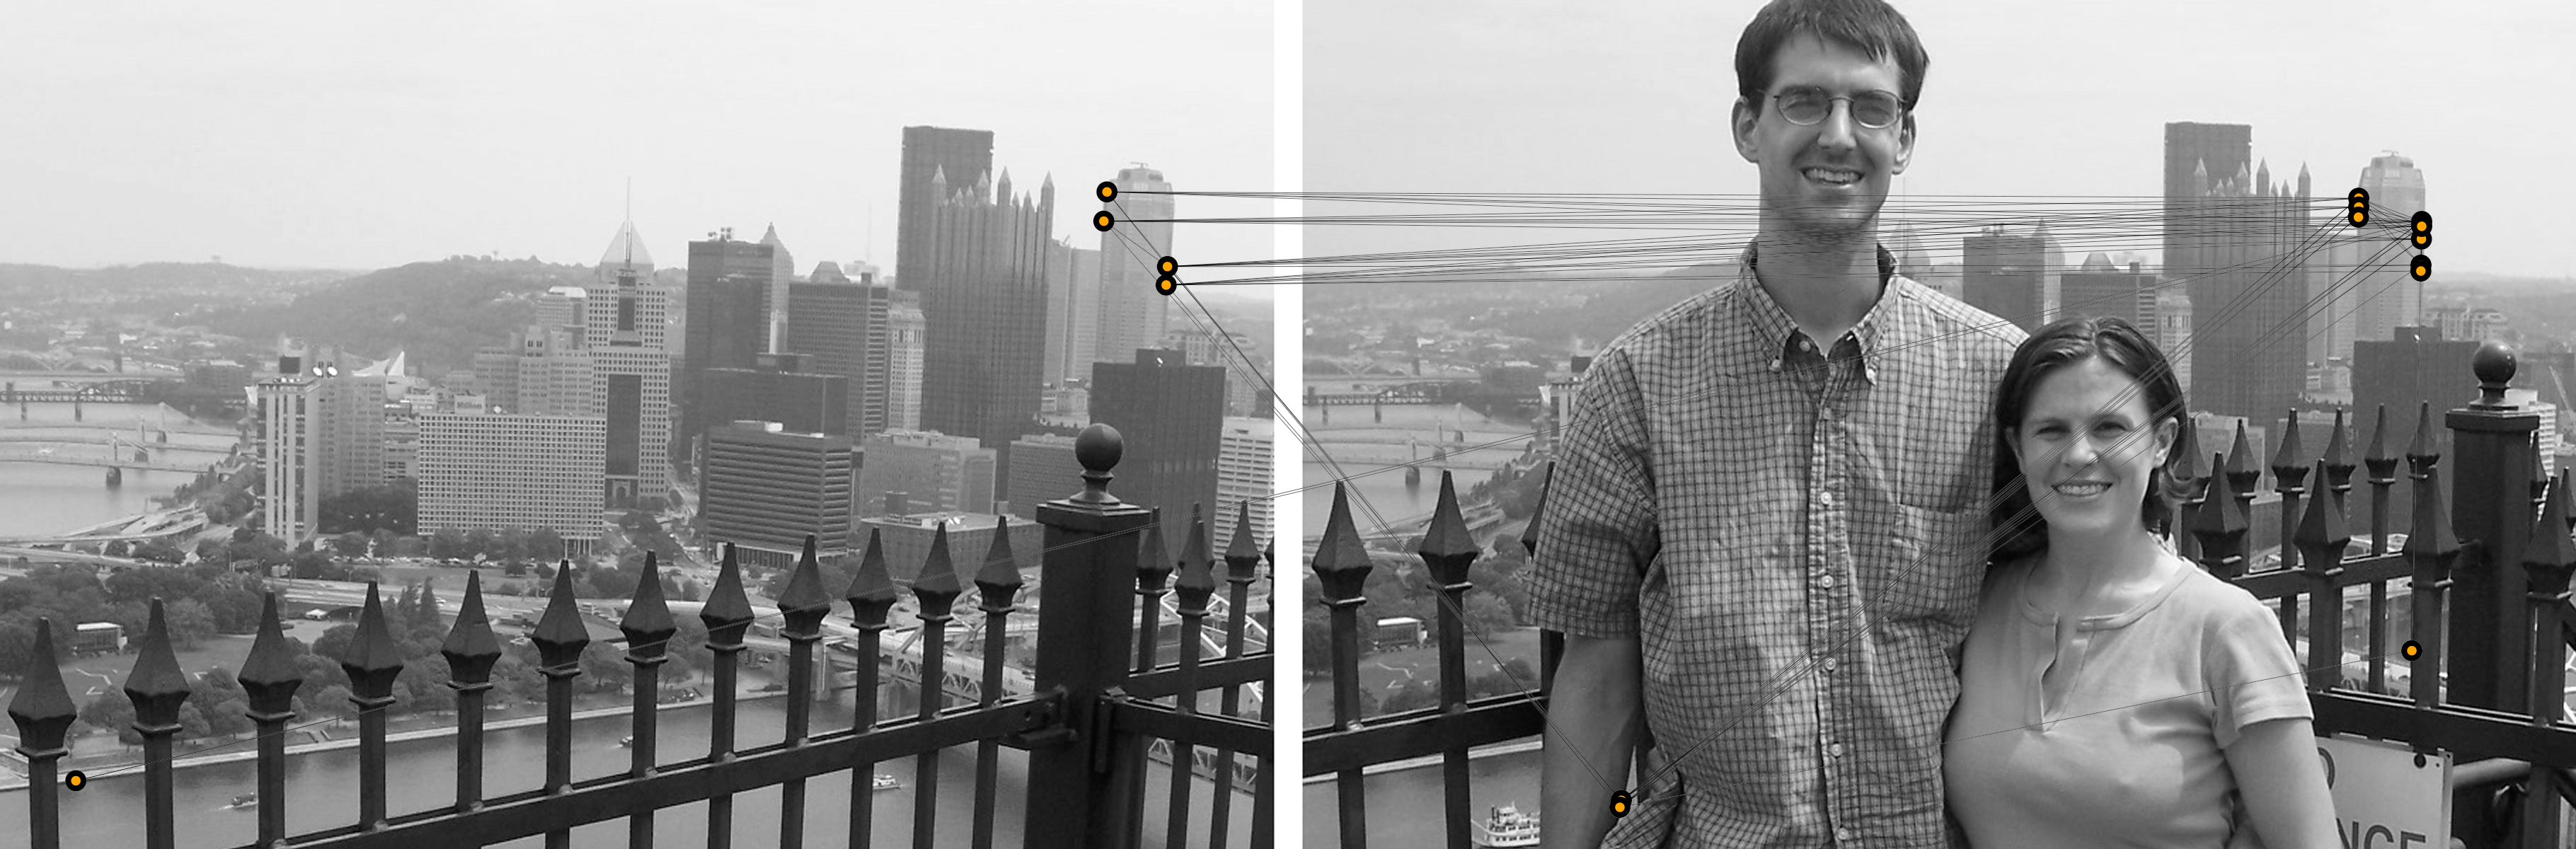
\includegraphics[width=0.85\columnwidth]{images/MMC_partition}
			\caption{\emph{MMC} Partition Example}
			\label{fig:pitts_partition}
		\end{subfigure}%
    \caption{Feature matching with \emph{MM} and \emph{MMC}. Dots 
        represent feature points; green/red lines indicate 
        correct/incorrect matches, respectively; black lines represent 
        edges in the feature graph.  (c) Result of \emph{NN-Ratio} 
        matching.  (d) All matches found by \emph{MM}, including 
        intra-image matches.  (e) Final \emph{MM} result.  (f) Example 
        of a partition of feature points after clustering, which 
        includes similar feature points from the same building across 
    both images.}%
	\label{fig:comparemirror}%
\end{figure}%

The central idea behind \emph{MM} is to match features of $n$ images by 
taking every feature from all $n$ images and matching them against every 
other feature from the same set. We can then discard the correspondences 
that match two points within the same image. Algorithm~\ref{alg-mm} 
details  the implementation of \emph{MM}.
%
\begin{algorithm}[htb]
\caption{Mirror Match (\emph{MM})}
\label{alg-mm}
\begin{algorithmic}
\Require $images$ : set of images, $t \in \mathbb{R}$
\State $M_{init}\gets \varnothing$, $M_{final}\gets 
\varnothing$, $F\gets \varnothing$
\ForAll{$I_i \in images$} \Comment Acquisition Stage
	\State $F\gets F \cup getF(I_i)$
\EndFor
\ForAll{$f_i \in F$} \Comment Matching Stage
    \State $f_m,f_n \gets get2NearestNeighbors(f_i, F \setminus 
    \left\{f_i\right\})$
    \State $ratio \gets distance(f_i, f_m) / distance(f_i, f_n)$
	\If{$ratio < t$}
		\State $M_{init} \gets M_{init} \cup \left(f_i, f_m\right)$
	\EndIf
\EndFor
\ForAll{$\left(f_i, f_j \right) \in M_{init}$} \Comment Filter 
Stage
\If{$\left(f_j, f_i \right) \in M_{init} \wedge getImg(f_i) \neq 
getImg(f_j) \wedge \left(f_j, f_i\right) \not\in M_{final}$}
		\State $M_{final} \gets (f_i, f_j)$
	\EndIf
\EndFor \\
\Return $M_{final}$
\end{algorithmic}
\end{algorithm}
%
In the acquisition stage we gather all features in the set of images.  
In the matching stage these features are matched using $k$-nearest 
neighbors.  For any given feature $f_i$ the two most similar neighbors 
are returned, and we calculate the ratio between them as proposed in 
\cite{lowe2004sift}.  Any correspondence with a ratio above the 
threshold supplied will be discarded. Finally in the filter stage we 
check that matches are from different images and discard all matches 
that are not symmetric.

Figure~\ref{fig:comparemirror} illustrates the benefits of \emph{MM} 
using an example image pair from the Gallagher dataset 
\cite{gallagher2008}.
With \emph{NN-Ratio} (Figure~\ref{fig:unique}), many incorrect matches 
occur in the fence towards the bottom of the image.
When we match all feature points together, many of these incorrect 
matches are eliminated, because points in the fence match with other 
points in the fence in the same image (Figures~\ref{fig:within} 
and~\ref{fig:without}).
%
\subsection{Mirror Match with Clustering (\emph{MMC})}
%
In contrast to \emph{MM}, \emph{MMC} diverges from traditional 
non-geometric feature matching by clustering feature points by 
similarity. This process yields partitions of fairly similar feature 
points that we can match using the same approach as \emph{MM}.  
Algorithm~\ref{alg-mmc} shows the pseudocode implementation of \emph{MMC}.
%
\begin{algorithm}[htb]
\caption{Mirror Match with Clustering (\emph{MMC})}
\label{alg-mmc}
\begin{algorithmic}
\Require $images$ : set of images, $t \in \mathbb{R}$, $\alpha \in 
\mathbb{R}$
\State $M\gets \varnothing$, $F\gets \varnothing$
\ForAll{$I_i \in images$} \Comment Gather features
    \State $F\gets F \cup getFeatures(I_i)$
\EndFor
\State $A\gets getAdjacencyMatrix(f_1, f_2,\; \ldots \;, f_n)$
\State $A_{norm}\gets normalize(A)$
\ForAll{$(i,j) \in indices(A)$} \Comment Prune edges
    \If{$A_{norm}[i,j] < \alpha$}
        \State $A_{norm}[i,j] \gets 0$
    \EndIf
\EndFor
\State $P\gets cluster(A_{norm})$
\ForAll{$p \in P$} \Comment p is a set of feature points
    \State $M\gets M \cup getMatches(p, t, F)$
\EndFor \\
\Return matches
\end{algorithmic}
\end{algorithm}
%
\begin{figure}[h]
	\centering
    \includegraphics[width=0.7\columnwidth]{images/MMC_graph_vert}
    \caption{The partitioned feature graph. Each vertex represents a 
        feature point; lines indicate high similarity between points. A 
        partition is a connected group with the same color. The border 
        color of each node indicates which image it belongs to.  Zooming 
    into a section of the graph, the various cluster sizes can be seen, 
ranging from hundreds of feature points to only two or three.}
	\label{fig:graph}
\end{figure}

We use the Louvain Method \cite{blondel2008} for clustering feature 
points, since it is relatively fast and performs 
well \cite{lancichinetti2009}, does not require 
parameters \cite{blondel2008}, and does not emphasize partitions of equal 
size, as opposed to spectral clustering or 
k-means \cite{von2007}, for example.
While the Louvain clustering algorithm does not require any parameters in 
itself, it tends towards clustering all feature points together in the 
same partition if the graph is very connected.  To ensure that the graph 
is well clustered, the adjacency matrix is pruned so that only edges above a 
certain threshold are kept. From empirical analysis, retaining the top 
2.5\% of edges with the highest similarity seems to work well in 
practice. Figure~\ref{fig:graph} shows the result of clustering the 
feature points as a graph.

The partitions group feature points by similarity, which means that 
repetitive structures such as buildings often appear in larger 
partitions, as exemplified in Figure~\ref{fig:pitts_partition}.

The matching algorithm for \emph{MMC}, \emph{getMatches}, finds matches 
within all partitions with more than two elements using the \emph{MM} 
approach.  However, as can be seen in the example in 
Figure~\ref{fig:graph}, many of the partitions contain only two feature 
points from different images linked by one edge. In such a case, we 
compare the similarity of the these two feature points with their second 
best match and remove matches where this ratio lies above a certain 
threshold, like in the \emph{NN-Ratio} algorithm. For example in the 
case of Figure~\ref{fig:pitts_partition}, we have several feature points 
from a building in one image grouped together with points from the same 
building in another image.
%
\section{Experiments}
\label{S:Experiments}
%
To reliably measure the accuracy of a matching method on real images, we 
either need a set of image pairs tied by a homography, or we have to manually count 
the number of inliers. The latter becomes prohibitive for large numbers of (non-trivial) images. 

Mikolajczyk and Schmid  \cite{mikolajczyk2005performance} introduced a set of test images
to compare the performance of feature detectors. The 
set covers different types of image variations, such as lighting change, 
blur, rotation, and viewpoint change. Inspired by this 
dataset (in particular the `Graf' image set) and motivated by 
the need for more image pairs featuring viewpoint changes, we have 
compiled a set of 8 image pairs consisting of subjects taken from two 
different angles. The images are collected from Flickr's database of 
images published under a creative commons licence and feature murals, 
which makes it possible to relate points in the image pairs with a 
homography.  The images have been cropped to show the same motive and 
resized to $900\times 600$ pixels.  This dataset will be referred to as 
the \emph{Murals} dataset.  Figure~\ref{fig:murals} shows one image from 
each pair.

\begin{figure}[htb]
%	\makebox[0.5\textwidth][c]{%
%		\begin{subfigure}[t]{0.048\textwidth}
%			\centering
%			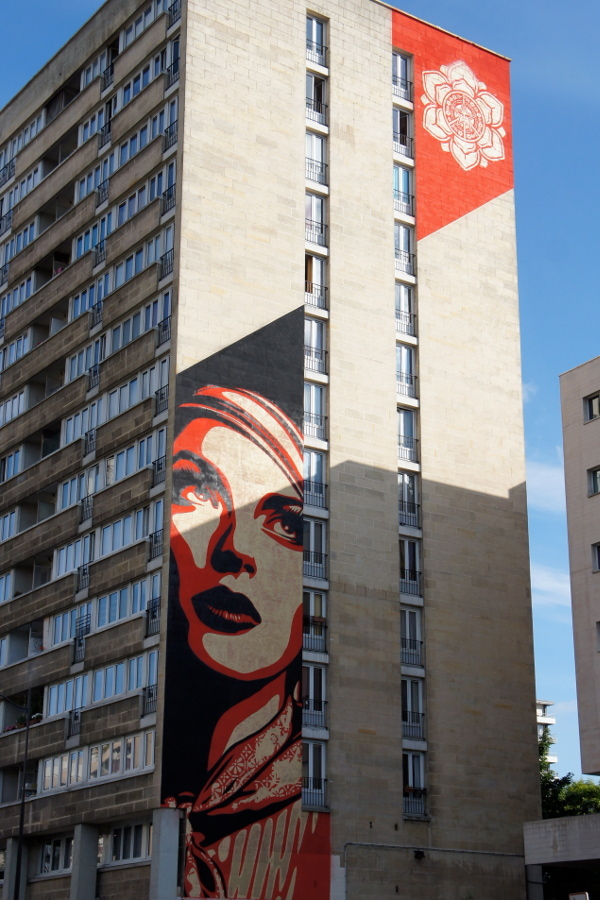
\includegraphics[width=\textwidth]{images/pair_example1}
%			\label{fig:fairey1}
%	\end{subfigure}%
%		\enspace %add desired spacing between images, e. g. ~, \quad, 
%		%(or a blank line to force the subfigure onto a new line)
%		\begin{subfigure}[t]{0.048\textwidth}
%			\centering
%			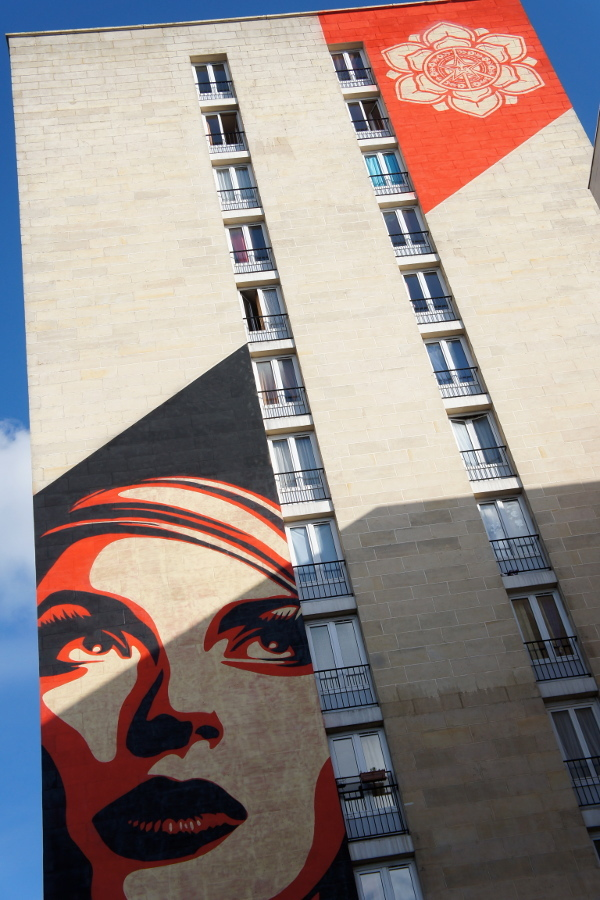
\includegraphics[width=\textwidth]{images/pair_example2}
%			\label{fig:fairey2}
%		\end{subfigure}%
%		\enspace %
%		\begin{subfigure}[t]{0.36\textwidth}
			\centering
			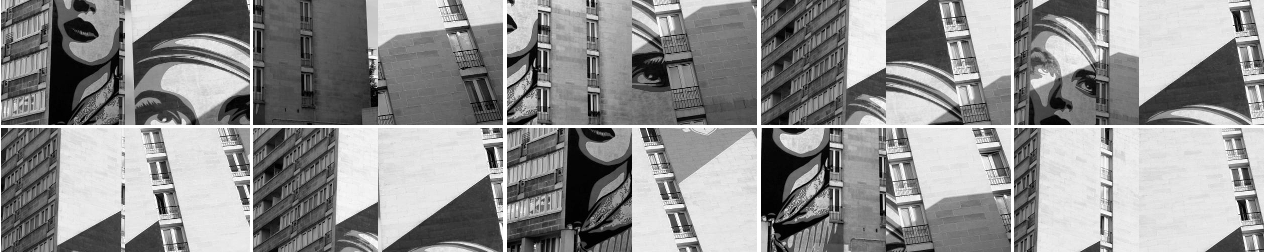
\includegraphics[width=\columnwidth]{images/crop_examples}
%		\end{subfigure}%
%	}%
	\caption{Sample test patches produced from an image pair.}
	\label{fig:fairey}
\end{figure}

\begin{figure*}[t]
	\centering
	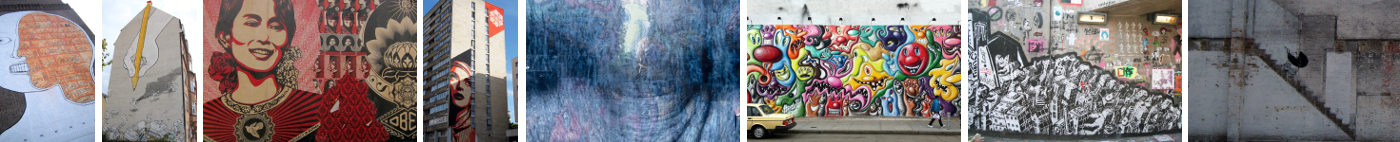
\includegraphics[width=\textwidth]{images/murals}
	\caption{Images in the \emph{Murals} test set.}
	\label{fig:murals}
\end{figure*}

\begin{figure}[htb]
	\centering
	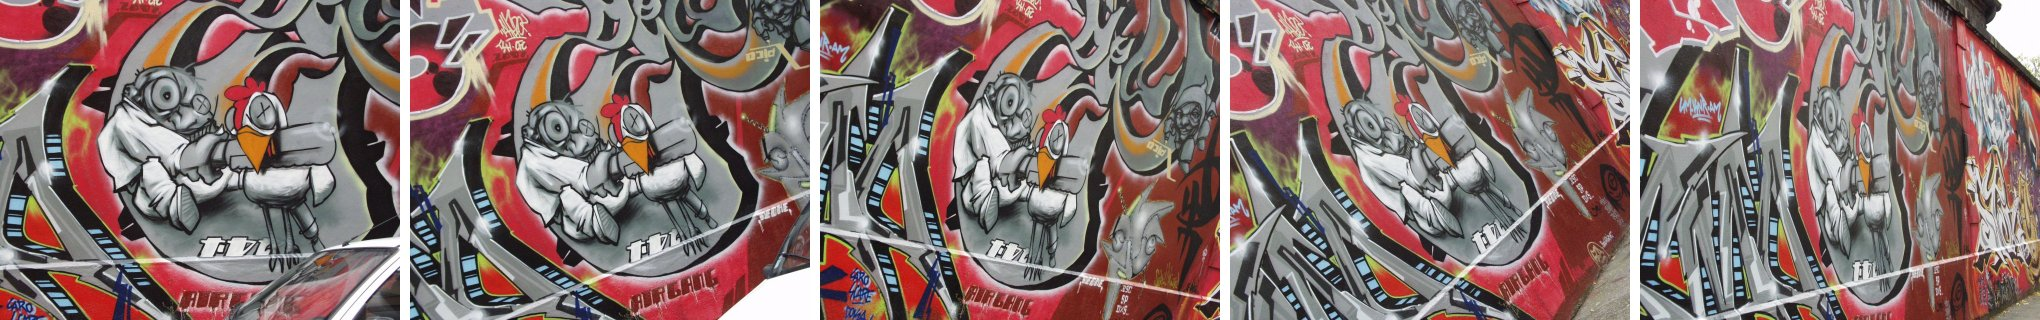
\includegraphics[width=\columnwidth]{images/graf12345.jpg}
	\caption{Images 1-5 of the Graf set from \cite{mikolajczyk2005performance}.}
	\label{fig:Graf}
\end{figure}


%However in practice the view point change has gone on to be used the 
%most for later tests given that most of the other test pairs have since 
%become easy to match\footnote{see \cite{wu2011robust} or 
%\cite{delponte2006svd} for examples}.

%Inspired by the graffiti image we have collected a set of image pairs 
%featuring murals of a few different artists\footnote{Including Banksy, 
%Blu and Shepard Fairey among others}. Each pair consist of images of 
%the same motive taken from different angles, often including repetitive 
%patterns and texture. Based on this image set the two algorithms are 
%tested on a series of image patches from each pair. To verify that the 
%algorithms proposed are reliable we need to test that we get good 
%matches when images overlap and that we get no matches when they do 
%not.  This means that it isn't enough just testing against pairs of 
%images that we know match.  We also need to test against pairs that 
%might look like they could match but in fact do not.


%
%
%\subsection{Experimental setup}
We compare the \emph{MM} and \emph{MMC} algorithms to \emph{NN-Ratio} 
\cite{lowe2004sift} as well as \emph{Isodata} \cite{das2008event} and 
\emph{Spectral} \cite{leordeanu2005spectral}.  \emph{Isodata} and 
\emph{Spectral} use geometric constraints, whereas \emph{NN-Ratio} does 
not.
%, which uses geometric information to improve the matching.  The 
%comparison  with \emph{NN-Ratio} serves to illustrate the relative 
%performance of \emph{MM} and \emph{MMC} to a state of the art algorithm 
%without geometric constraints. \emph{Isodata} is included to illustrate 
%the performance of an algorithm relying on geometric constraints faced 
%with image pairs that might not have any overlap.  
The comparison was done using the \emph{Murals} dataset 
(Figure~\ref{fig:murals}), the \emph{Graf} set (Figure~\ref{fig:Graf}) 
from \cite{mikolajczyk2005performance}, and two images 
%\footnote{100\_1942.jpg and 100\_1941.jpg} from the Gallagher dataset 
%\cite{gallagher2008} (Figure~\ref{fig:comparemirror}).

Test sets were generated from the image pairs by cropping square patches of
$250\!\times\!250$ pixels with a random vertical and horizontal offset.  
Given a source image pair, we produce 100 pairs of patches, which might or might not overlap.  
This ensures that patch pairs with no overlap still retain a general similarity to each 
other, while patches that do overlap often only share a small 
part of their area. Figure~\ref{fig:fairey} shows an example of 
possible pairs of test image patches produced from a source image pair.  
Producing $n$ such pairs allows us to test not just how well the 
matching algorithm performs on a variety of overlaps but also how many 
false positives we get on similar images that do not 
overlap.\footnote{~The set of source images and homographies as well as 
the script to generate the cropped test sets based on them can be found 
at 
\href{http://vintage.winklerbros.net/murals.html}{http://vintage.winklerbros.net/murals.html}}.  
In practice the amount of overlap between pairs in a test set will 
depend on the overlap and viewpoint change in the source image pair.  To 
give a rough idea, Table~\ref{table:overlap} shows the overlap of patch 
pairs created from images 1 and 3 of the \emph{Graf} image set from 
\cite{mikolajczyk2005performance}.

\begin{table}[htb]
\caption{Overlap in the set of 100 patch pairs created from two images of the \emph{Graf} image set (Figure~\ref{fig:Graf}).}
\label{table:overlap}
	\centering
%	\small
\begin{tabular}{r*{3}{r}}
\hline
	Amount of overlap: & 0\% & $< 50$\% & $> 50$\%  \\
	\noalign{\smallskip}
	%
	Number of patch pairs: & 21 & 54 & 25 \\
	\hline
\end{tabular}
\end{table}


Given a potential match between two pixels $p_1$ and 
$p_2$, $m = \left(p_1, p_2\right)$, and a homography $H$ relating the two images $I_1$ and $I_2$, we 
can calculate if $m$ is an inlier by checking if the two points satisfy the following criteria:
\begin{equation*}
\left\vert H p_1 - p_2 \right\vert + \left\vert H^{-1}p_2 - p_1 \right\vert < d_{\max}
\end{equation*}
That is, the distance between $p_1$ translated to $I_2$ and $p_2$ 
\emph{plus} the distance between $p_2$ translated to $I_1$ should be 
less than a certain threshold (we use $d_{\max}=5$ pixels here).


\section{Results}
\label{S:Results}

Figure~\ref{fig:result_graf} shows the results for 100 patch pairs 
generated from images 1 and 3 of the \emph{Graf} image set 
(cf.~Figure~\ref{fig:Graf}). We plot the precision and recall of 
\emph{MMC}, \emph{MM}, \emph{Isodata}, \emph{Spectral} and 
\emph{NN-Ratio}. The precision and recall is calculated as follows:

\begin{equation*}
    Precision = \frac{\# ~ Correct ~ Matches}{\# ~ Correct ~ Matches ~ + 
    ~ \# ~ False ~ Matches} \\
\end{equation*}
\begin{equation*}
    Recall = \frac{\# ~ Correct ~ Matches}{\# ~ Total ~ Possible ~
    Matches}
\end{equation*}

The plot data is obtained by varying ratio thresholds.  The results show 
that \emph{MM} and \emph{MMC} consistently outperform \emph{NN-Ratio}; 
\emph{MMC} generally lies 2-3 percentage points above \emph{MM} when 
both are performing at optimal accuracy.  Although \emph{Isodata} and 
\emph{Spectral} exhibits a good performance on strict thresholds (small 
number of matches), that quickly diminishes when more matches are 
desired.

\begin{figure}[htb]
%	\makebox[0.5\textwidth][c]{%
%		\begin{subfigure}[t]{.13\textwidth}
%			\centering
%			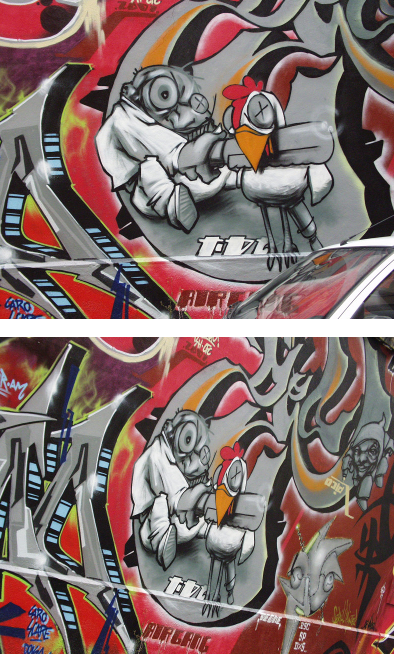
\includegraphics[width=\textwidth]{images/graf}
%		\end{subfigure}%
%		~ %add desired spacing between images, e. g. ~, \quad, \qquad		  
		%(or a blank line to force the subfigure onto a new line)
%		\begin{subfigure}[t]{.27\textwidth}
			\centering
            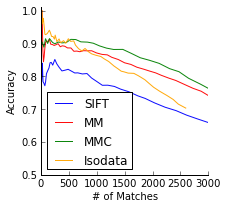
\includegraphics[width=0.8\columnwidth]{images/result_graf}
			%\caption{Performance on Scharf}
%		\end{subfigure}%
%	}%
	\caption{Accuracy for image pair 1\&3 from the \emph{Graf} set. The plot 
		shows the result of 100 patch pairs generated from the source 
		images shown to the left. The number of matches is the total 
		number of matches for all 100 patch pairs.}
	\label{fig:result_graf}
\end{figure}

To validate whether these results generalize to other images, we tested 
the five algorithms on the \emph{Murals} dataset as well as the 
\emph{Graf} pair tested above.  In total 900 different patch pairs were 
generated from 9 source image pairs.  The results are shown in Figure 
\ref{fig:result_accumulated}. 

\begin{figure}[htb]
	\centering
    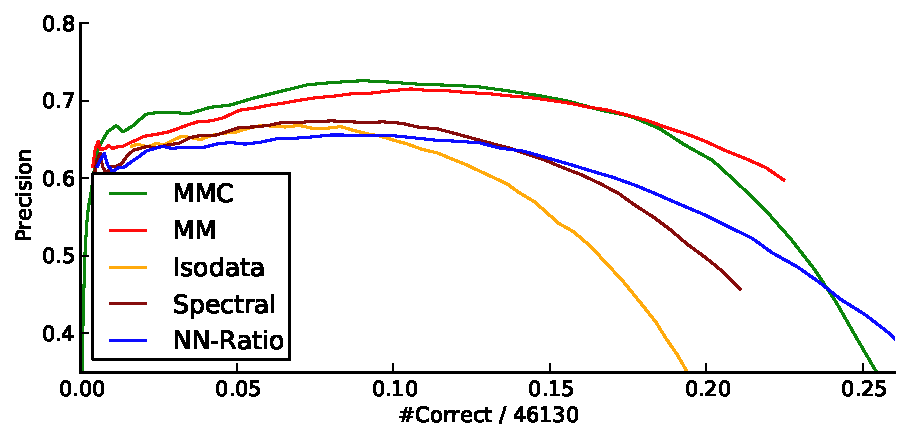
\includegraphics[width=0.8\columnwidth]{images/result_accumulated}
	\caption{Results for 900 patch pairs extracted from the \emph{Murals} dataset and the image pair 1\&3 from the \emph{Graf} set.  The x-axis shows the accumulated returned matches for all pairs.}
	\label{fig:result_accumulated}
\end{figure}

To further investigate the impact of viewpoint changes, we tested the 
algorithms on the \emph{Graf} image set (Figure~\ref{fig:Graf}), which 
contains 5 images of the same mural taken with gradually increasing 
viewpoint changes.  The first images are almost identical, while the 
last are taken from very different angles. The results from   \emph{MMC} 
and \emph{NN-Ratio} as shown in Figure~\ref{fig:result_viewpoint}, 
confirming that \emph{MMC} is generally superior to \emph{NN-Ratio} 
across viewpoint changes.
The performance of \emph{MM} (not shown in the plot) is similar to 
\emph{MMC}.

\begin{figure}[htb]
	\centering
    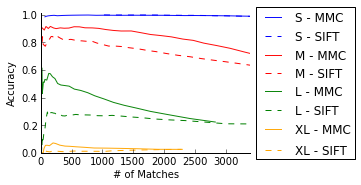
\includegraphics[width=0.8\columnwidth]{images/result_viewpoint}
	\caption{Results for viewpoint changes using the \emph{Graf} set from 
		\cite{mikolajczyk2005performance}.  S: img1\&2; M: img1\&3; L: img1\&4; XL: img1\&5.}
	\label{fig:result_viewpoint}
\end{figure}

Finally, for an example of a real life use case, 
Figure~\ref{fig:result_pitts} shows the results on 100 patch pairs 
generated from a typical holiday photo shot 
(Figure~\ref{fig:pitts_source}) featuring occlusion and a slight 
viewpoint change from the Gallagher dataset \cite{gallagher2008}.  The 
performance is comparable to the murals, despite the lack of a simple 
homographic mapping between the images.

\begin{figure}[htb]
\centering
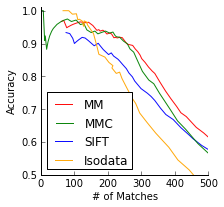
\includegraphics[width=0.8\columnwidth]{images/result_pitts}
\caption{Results for the image pair in Figure~\ref{fig:pitts_source}.}
\label{fig:result_pitts}
\end{figure}

In terms of computational complexity, \emph{NN-Ratio}, \emph{MM}, and 
\emph{Isodata} can be implemented in $O(n\log n)$, where $n$ is the 
total number of feature points.  \emph{Spectral} and our current 
\emph{MMC} implementation has a complexity of $O(n^2)$ due to the 
construction of a similarity matrix of the feature points. However, both
can be approximated in $O(n\log n)$ using search trees to sparsely 
populate the adjacency matrix.  

In terms of speed, Table~\ref{table:running_times} shows the 
running time of the four algorithms over 100 image pairs of $250\!\times\!250$ pixels. 
These numbers should be taken with a grain of salt, given that 
much of the code behind \emph{MMC} and \emph{Isodata} is implemented in 
Python, whereas \emph{MM} and \emph{NN-Ratio} make use of OpenCV to 
execute computationally intensive operations in C++, which makes them 
much faster. 

\begin{table}[htb]
\caption{Running times as tested on a Intel\textregistered\ Core\texttrademark\ i5-3550 CPU @ 
3.30~GHz with 8~GB memory.}
\label{table:running_times}
	\centering
%	\small
\begin{tabular}{r*{5}{c}}
\hline
	Algorithm: & \emph{Ratio} & \emph{MM} & \emph{MMC} %
& \emph{Isomatch} & \emph{Spectral}	\\
	\noalign{\smallskip} 
	%
	Running time (seconds): & 21 & 23 & 2722 & 1146 & 994\\
	\hline
\end{tabular}
\end{table}
%

\section{Summary}
\label{S:Summary}

We have addressed the problem of matching feature points without using 
geometrical constraints, proposing \emph{Mirror Match 
(MM)} and \emph{Mirror Match with Clustering (MMC)}.  The two algorithms 
share the common idea that feature points should have better 
matches in another image than in the image they came from to be 
considered good matches.  \emph{MMC} further improves on this idea by 
using the structure of the similarity graph of the feature points. 

The algorithms show promising results when tested on the \emph{Murals} 
data set. \emph{MM} and \emph{MMC} generally outperform existing 
matching algorithms \emph{NN-Ratio} and \emph{Isodata}, and \emph{MMC} 
outperforms \emph{MM}. We show that this result generalizes to 
variations in viewpoint change as well as more realistic photos 
featuring occlusions. 

Given the versatility of the proposed algorithms, we are planning to 
apply them to problems that require high reliability faced with images 
that might not match, such as near duplicate detection or face 
recognition.

\textit{This work is supported by the research grant for ADSC's Human 
Sixth Sense Programme from Singapore's Agency for Science, Technology 
and Research ($\text{A}^\star$STAR).}
%
\bibliographystyle{IEEEtran}
\bibliography{tail/bibliography}
\end{document}
